% ============================================================================
% Paste-ready supplement for Model III (replaces the two TODO placeholders in
% model3.tex). Style, labels and notation follow the joint report:
%   \mathcal{G}(i) genre map, \cref cross-references, booktabs tables.
% Figure file required: genre_influence_over_time.pdf (panel (a)(b), compact,
%   sits next to \cref{fig:q3-pair-time}).
% ============================================================================

\subsection{How Genre Influence Changes over Time}\label{subsec:q3-inf-time}

While \cref{subsec:q3-sim-time} tracks how \emph{sonic similarity} between
genres evolves, this subsection quantifies how \emph{reported influence}
between genres evolves. We do not build a second network: the genre-level
flows are obtained by \emph{aggregating} the artist-level network of
Model~I over the genre partition, exactly as the Katz-weighted centroids
of \cref{subsec:q3-centroids} aggregate the feature vectors. For each pair
of main genres $(g,h)$ we count
\begin{equation}\label{eq:F-gh}
F_{gh} \;=\; \sum_{(i,j)\in E}\,
\mathbb{1}\!\left[\mathcal{G}(i)=g\right]\,
\mathbb{1}\!\left[\mathcal{G}(j)=h\right],
\end{equation}
the number of reported edges from genre-$g$ influencers to genre-$h$
followers. The construction is a deterministic group-by on the cleaned
edge table of section~4.2, so it introduces no new edge definition and no
new parameters. Its correctness is guaranteed by the conservation identity
$\sum_{g,h}F_{gh}=|E|=42{,}770$ (including the $733$ time-reversed edges
retained under Assumption~A3; excluding them gives $42{,}037$), which we
verify explicitly, and by an exact match of the Jazz$\to$Pop/Rock block
with the subnetwork count of section~5.6 ($409$ edges; $406$ when the
three reversed edges among them are excluded). All counts in this
subsection follow the same convention. Row- and column-normalized variants,
$P_{gh}=F_{gh}\big/\sum_{h'}F_{gh'}$ and
$Q_{gh}=F_{gh}\big/\sum_{g'}F_{g'h}$, express the \emph{export profile} of
$g$ and the \emph{source profile} of $h$; the normalization removes the
strong size effect of the genre labels (Pop/Rock alone carries $56\%$ of
all edges, section~4.4) and leaves pure flow structure.

The time dimension follows the cohort convention of section~5.5:
$F_{gh}(t)$ restricts \eqref{eq:F-gh} to edges whose \emph{follower}
started in decade $t$ (1930--2010; decades with fewer than $50$ edges are
omitted). As in \cref{subsec:q3-sim-time} we treat 1950--2000 as the main
window; the 1930s and 2010s cohorts are thin (193 and 811 edges) and are
read only with that caveat. We emphasize that this conditioning variable
differs from
\cref{subsec:q3-sim-time}, which indexes artists by their \emph{own}
active-start decade: there $\mathbf{c}_g(t)$ describes the sound of genre
$g$'s generation $t$, here $F(t)$ describes what generation $t$
\emph{absorbed}. The two curves of \cref{fig:q3-pair-time} and
\cref{fig:q3-inf-time} are therefore complementary readings of the same
timeline.

\paragraph{Cross-genre influence rises, peaks, and settles into a
plateau.} Let
$c(t)=1-\sum_g F_{gg}(t)\big/\sum_{g,h}F_{gh}(t)$ denote the cross-genre
share of edges received by generation $t$ (panel~(a) of
\cref{fig:q3-inf-time}). The share climbs from $0.23$ (1940s cohort) to a
peak of $0.37$ for the 1960s cohort---the era in which Blues, R\&B,
Country and Pop/Rock most heavily cross-fed, consistent with the birth of
rock---and then falls to a stable plateau of $0.18$ across the
1980s--2000s cohorts (the thin 2010 cohort ticks up to $0.23$). In terms
of raw reported edges, later generations drew an increasingly
\emph{within-genre} diet.

\paragraph{Quantity and quality of cross-genre influence diverge.} The raw
share treats all followers equally. Re-weighting each edge by the
follower's outgoing Katz score $K_j$ from Model~I---influencing a future
hub counts for more---produces the Katz-weighted share $c_K(t)$ (blue
dashed curve of panel~(a)). Its maximum shifts a full decade earlier:
$c_K(t)$ peaks at $0.53$ for the 1950s cohort and collapses below $0.19$
for every cohort from the 1970s through the 2000s (the thin 2010 cohort
ticks back up to $0.23$). The divergence between the two curves is itself
informative: among early post-war artists, those who absorbed cross-genre
influence went on to become disproportionately influential themselves,
whereas among artists active from the 1970s onward, cross-genre followers
are on average \emph{less} connected to future influence than same-genre
followers. The era of maximum cross-genre \emph{traffic} (1960s) precedes
the era of maximum cross-genre \emph{leverage} (1950s).

\paragraph{Selected flows.} Panel~(b) plots the export share $P_{gh}(t)$
for five informative pairs (genre-decade rows with at least $20$ edges are
shown). Three patterns stand out.
(i)~\emph{Jazz steadily redirects its influence outward}: its export share
toward Pop/Rock rises overall from $0.05$ (1950s cohort) to $0.35$ (2000s
cohort)---holding at $0.20$--$0.23$ across the 1960s--1980s cohorts with a
dip to $0.20$ in the 1990s---while the Jazz$\to$Jazz block
shrinks---jazz increasingly feeds mainstream genres rather than its own
tradition. (The 2010 cohort is omitted from panel~(b): it contains only
three Jazz edges.)
(ii)~\emph{Blues--R\&B decouples}: Blues' export share toward R\&B is
$0.23$ for the 1930s cohort---five edges, out of an R\&B inflow of just
seven, so Blues supplied $71\%$ of everything the first R\&B cohort
received---but the share falls below $0.16$ already in the 1940s and to
$0$--$6\%$ across the 1980s--1990s cohorts (on $41$--$78$ edges); what
remains afterwards is small-sample noise ($0.19$ in the 2000 cohort
represents four edges). The pattern reflects the diversification of R\&B's
sources as the genre broadened.
(iii)~\emph{Electronic enters late and feeds Pop/Rock strongly}: the flow
only appears in the 1970s (the genre itself barely exists before then) and
immediately dominates Electronic's export profile ($0.70$ for the 1970s
cohort, $0.50$ for the 2000s cohort).

\paragraph{Where similarity and influence move together or diverge.}
Reading \cref{fig:q3-inf-time} against \cref{fig:q3-pair-time} shows that
the two lenses agree only partially.
\emph{Together}: Electronic--Pop/Rock both converges in sound
($\Delta s\approx+0.18$ in \cref{subsec:q3-sim-time}) and dominates
Electronic's export profile---sonic convergence here tracks reported
influence.
\emph{Diverging, influence ahead of sound}: Jazz's export share toward
Pop/Rock rises overall ($0.05\to0.35$, with a 1990s dip) while the
Jazz--Pop/Rock
similarity stays flat or drifts slightly down ($0.25\to0.23$); reported
influence deepened even as the two profiles drifted apart.
\emph{Diverging, influence behind sound}: Blues--R\&B is the sonically
closest pair of the whole system ($d=0.76$ in \cref{subsec:q3-centroids}),
yet Blues' export share toward R\&B fell from $0.23$ to $0$--$6\%$ across
the 1980s--1990s cohorts; closeness of sound did not preserve closeness of
reported influence.
Sonic similarity is thus neither necessary nor sufficient for reported
influence---the two measures answer different questions, which is why we
keep both.

\paragraph{Where the influence mass sits.} A complementary,
follower-independent view aggregates the artists themselves:
$K_g(t)=\big(\textstyle\sum_{i:\,\mathcal{G}(i)=g,\,
\mathrm{start}(i)=t}K_i\big)\big/
\big(\textstyle\sum_{i:\,\mathrm{start}(i)=t}K_i\big)$, the share of
generation $t$'s outgoing-Katz mass held by genre $g$. Pop/Rock rises from
negligible mass in the 1930s to $0.73$--$0.75$ for the 1960s--1980s
cohorts and remains dominant; Jazz collapses from $0.24$ (1930s) to
$0.01$ (1980s onward); Electronic grows from zero to ${\approx}\,0.08$.
The genre system concentrated its influence-carrying capacity into
Pop/Rock precisely during the decades in which its cross-genre
\emph{intake} fell---consolidation of output accompanied consolidation of
input.

\begin{figure}[htbp]
\centering
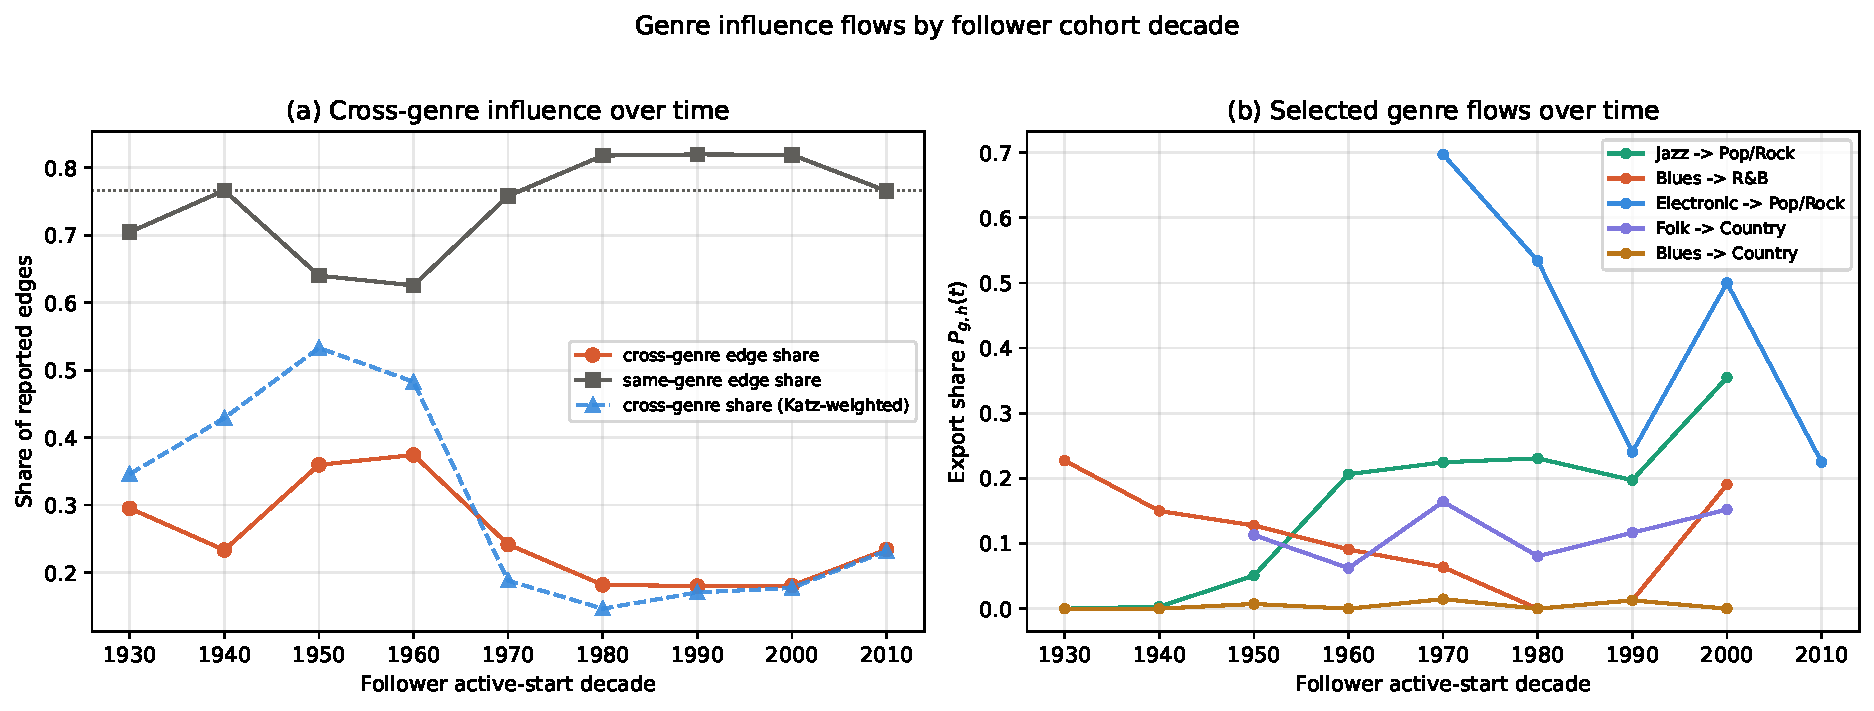
\includegraphics[width=0.98\textwidth]{genre_influence_over_time.pdf}
\caption{Genre influence flows by follower cohort decade.
(a)~Cross-genre share of edges $c(t)$ (red) against the same-genre share
(grey; dotted line marks the all-network value $0.766$), and the
Katz-weighted cross-genre share $c_K(t)$ (blue dashed).
(b)~Export share $P_{gh}(t)$ for five selected flows; points are shown
only for genre-decade rows with at least $20$ edges.}
\label{fig:q3-inf-time}
\end{figure}

\paragraph{Robustness and disclosure.} The matrices retain edges whose
labels are \texttt{Unknown} so that the conservation identity holds
exactly; the discussion above concerns the 19 named genres. Retaining the
733 time-reversed edges follows Assumption~A3, and their impact is
quantified in section~5.7; removing them changes the decade cross-genre
shares by at most $0.023$ (1930s cohort, the smallest sample) and by no
more than $0.01$ for every decade from the 1940s onward, so no conclusion
moves. The Katz-weighted curve $c_K(t)$ uses the same attenuation
$\alpha=0.10$ as Model~I; the artist-level attenuation scan of
section~5.7 (rank correlation ${\ge}\,0.975$ over
$\alpha\in[0.05,0.20]$) supports that reweighting with a different
$\alpha$ would not alter the shape of panel~(a).

Two significance checks back the shape of panel~(a). First, a
\emph{permutation test} addresses the concern that decade-to-decade moves
in $c_K(t)$ merely track the changing genre composition of each cohort:
within each decade we shuffle the influencer genre labels (1{,}000
draws), which keeps the cohort's edge count, genre mix and follower Katz
weights fixed while destroying any real genre homophily. Observed
$c_K(t)$ lies far \emph{below} the composition-adjusted null in every
cohort---genres are homophilous in whom they cite---but the excess
homophily is precisely what carries the story: it is weakest for the
1950s--1960s cohorts ($z\approx-10$ to $-21$) and strongest from the
1980s onward ($z\le-45$; all one-sided $p<0.001$). The mid-century peak
in cross-genre influence is therefore not an artifact of which genres
happened to be large at the time.

\subsection{Are Some Genres Related to Others?}\label{subsec:q3-related}

\cref{subsec:q3-centroids} supplies a \emph{sonic} relatedness picture
($d_{gh}$, \cref{fig:q3-genre-dist}); \cref{subsec:q3-inf-time} supplies a
\emph{reported-influence} picture ($F_{gh}$ and $P_{gh}$). Joining them
yields a simple typology of genre relatedness. A \emph{Mantel test}
correlating the off-diagonal entries of the sonic-distance matrix with
those of the symmetric cross-flow matrix ($F_{gh}+F_{hg}$,
log-scaled) gives $r=-0.41$ with permutation $p=0.0008$
($5{,}000$ row/column permutations): reported influence decays with sonic
distance, and every one of the strongest cross-links
(${\ge}\,200$ edges) lies at moderate distance
($1.2\le d\le 3.2$). Three regimes emerge
(\cref{tab:q3-related-types}).

\emph{(i)~Sonically close and strongly cross-linked.} Pop/Rock--R\&B
($d=1.23$, $1{,}909$ cross edges) is the dominant corridor of the whole
network, followed by Country--Pop/Rock ($2.06$; $1{,}160$),
Electronic--Pop/Rock ($2.42$; $801$), Blues--Pop/Rock ($1.79$; $736$) and
Latin--Pop/Rock ($1.19$; $235$). These are pairs whose sound is similar
\emph{and} whose artists cite each other heavily: relatedness in both
senses at once.

\emph{(ii)~Sonically close but weakly linked.} Blues--Country
($d=0.78$ but only $16$ cross edges), Latin--R\&B ($0.86$; $39$),
Country--R\&B ($1.09$; $46$) and Folk--Vocal ($1.06$; $19$) are sonic
siblings that rarely cite each other directly. Their resemblance is
plausibly a shared ancestry---both grew from common roots---rather than
an active exchange documented in the data.

\emph{(iii)~Sonically far yet influential---only in relative terms.} No
distant pair clears the $200$-edge bar: at the level of raw counts,
sonically remote genres barely interact. The share view
($Q_{gh}$) reveals a weaker form of the regime confined to niche genres
with thin inflows: Pop/Rock supplies $31\%$ of the (small) influence
received by Classical ($d=5.04$), and Pop/Rock dominates the inflows of
Avant-Garde ($30\%$, $d=7.84$) and New~Age ($19\%$, $d=5.00$). These are
cases where one mainstream donor towers over a shallow pool, not genuine
long-range channels.

The typology also exposes a strong \emph{hub asymmetry}: Pop/Rock
accounts for $45\%$ of everything Electronic receives, while the reverse
flow is $1.1\%$ of what Pop/Rock receives ($504$ vs.\ $297$ edges). In
the reported network, influence is not exchanged between equals---it is
donated by the hub, and the hub barely records what it takes in.

\begin{table}[htbp]
\centering
\small
\caption{Relatedness typology from sonic distance $d_{gh}$
(\cref{fig:q3-genre-dist}) and reported cross-genre edges
($F_{gh}+F_{hg}$). Type~(iii) examples are shown with the donor's share
$Q_{gh}$ of the receiver's inflow, since their absolute counts are small.}
\label{tab:q3-related-types}
\begin{tabular}{llrl}
\toprule
Type & Pair & $d_{gh}$ & Evidence \\
\midrule
(i) close \& strongly linked
  & Pop/Rock--R\&B        & $1.23$ & $1{,}909$ cross edges \\
  & Country--Pop/Rock     & $2.06$ & $1{,}160$ cross edges \\
  & Electronic--Pop/Rock  & $2.42$ & $801$ cross edges \\
  & Blues--Pop/Rock       & $1.79$ & $736$ cross edges \\
\addlinespace
(ii) close \& weakly linked
  & Blues--Country        & $0.78$ & $16$ cross edges \\
  & Latin--R\&B           & $0.86$ & $39$ cross edges \\
  & Country--R\&B         & $1.09$ & $46$ cross edges \\
\addlinespace
(iii) far \& influential (relative)
  & Pop/Rock $\to$ Classical    & $5.04$ & $31\%$ of inflow ($Q$) \\
  & Pop/Rock $\to$ Avant-Garde  & $7.84$ & $30\%$ of inflow ($Q$) \\
  & Pop/Rock $\to$ New Age      & $5.00$ & $19\%$ of inflow ($Q$) \\
\bottomrule
\end{tabular}
\end{table}
